\documentclass{beamer}
\usepackage{xcolor}
\usepackage{graphicx, subcaption}
\usepackage{tikz}
\usepackage{booktabs}

\usepackage{listings}
\lstset{
    language=Python,
    basicstyle=\ttfamily\scriptsize,
    keywordstyle=\color{blue}\bfseries,
    commentstyle=\color{green!50!black},
    stringstyle=\color{red!70!black},
    showstringspaces=false,
    breaklines=true,
    frame=single,
    columns=fullflexible
}


\usetikzlibrary{trees}

\usepackage{amsmath, amssymb, amsthm}

\title{MATH4907 Tutorial 1}
\author{Sanyang Liu}


\usetheme{Boadilla}
\useoutertheme{miniframes}
\setbeamertemplate{navigation symbols}{}

\newcommand{\bE}{\mathbb{E}}
\newcommand{\bQ}{\mathbb{Q}}
\newcommand{\bP}{\mathbb{P}}
\newcommand{\cF}{\mathcal{F}}



\begin{document}

\maketitle

\begin{frame}{Personal Information}
\begin{itemize}
    \item TA: Sanyang Liu
    \item Office: Room 320A Run Run Shaw Building (Email me first)
    \item Email: u3013241@connect.hku.hk
    \item Research interest: Numerical Methods for PDEs
    \\(PS \textcolor{red}{NOT} an expert for financial math!)
\end{itemize}
\end{frame}

\begin{frame}{Table of Contents}
    \tableofcontents
\end{frame}


\section[Intro]{Introduction}
\begin{frame}{Introduction}
We consider a financial market contains
\begin{itemize}
    \item a \textcolor{red}{riskless bond} $B_t$ with \textcolor{red}{interest rate} $r>0$ satisfy
    \begin{equation}
        B_t=B_0 e^{rt}
    \end{equation}
    \item an \textcolor{red}{underlying asset} $S_t$
    \item a \textcolor{red}{contingent claim} $V_t$ on the underlying asset $S_t$
\end{itemize}
\end{frame}

\section[BOPM]{Binomial Tree Model (Q1)}
\begin{frame}{Basic Settings}
    \begin{itemize}
        \item Inputs: $\big(S_0, T, V_T(S_T)\big)$
        \item Parameters: $(p, u, d,\textcolor{gray}{\Delta t})$
        \item Updating Rule:
        $\mathbb{P}[S_n=S_0u^id^{n-i}] = \binom{n}{i} p^i (1-p)^{n-i}$
        \item Outputs: $V_0$
    \end{itemize}
    \centering
    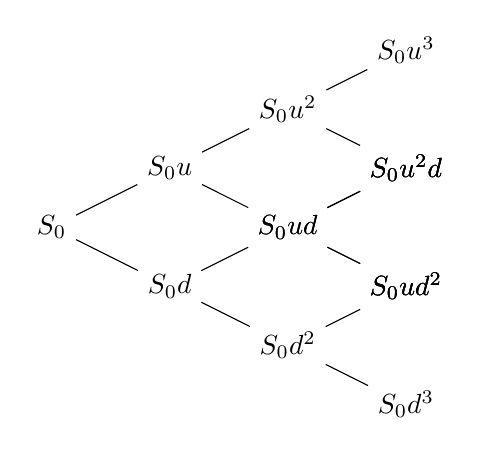
\begin{tikzpicture}[
    grow=right,
  level 1/.style={},
  level 2/.style={},
  level 3/.style={},
  every node/.style={}
]
\node {\(S_0\)}
  child { node {\(S_0d\)}
    child { node {\(S_0d^2\)}
      child { node {\(S_0d^3\)} }
      child { node {\(S_0ud^2\)} }
    }
    child { node {\(S_0ud\)}
      child { node {\(S_0ud^2\)} }
      child { node {\(S_0u^2d\)} }
    }
  }
  child { node {\(S_0u\)}
    child { node {\(S_0ud\)}
      child { node {\(S_0ud^2\)} }
      child { node {\(S_0u^2d\)} }
    }
    child { node {\(S_0u^2\)}
      child { node {\(S_0u^2d\)} }
      child { node {\(S_0u^3\)} }
    }
  };
\end{tikzpicture}
\end{frame}

\begin{frame}{Hedging portfolio}
\begin{block}{No-arbitrage assumption}
Two portfolios that have the same future payoff must have the same value today. Otherwise, an investor could make a risk-free profit with zero initial investment.
\end{block}
Consider the \textcolor{red}{hedge portfolio}
\[
\Pi_i:=V_i - \Delta S_i,
\]
where $\Delta$ is called the hedge ratio. We choose $\Delta$ to make $\Pi_i$ riskless, which could be priced using riskless bond $B_i$ (by no-arbitrage assumption).
\end{frame}

\begin{frame}{Risk neutral probability}
Then,
\begin{equation*}
    V_{i+1}(U) - \Delta S_{i+1}(U) = \Pi_{i+1}(U)\equiv\Pi_{i+1}(D) = V_{i+1}(D) - \Delta S_{i+1}(D).
\end{equation*}
It follows that
\[
\Delta = \frac{V_{i+1}(U) - V_{i+1}(D)}{S_i(u-d)}.
\]
By no-arbitrage assumption,
\[
\Pi_{i+1} = e^{r\Delta t}\Pi_i, \quad d<e^{r\Delta t} < u,
\]
and the price of the contingent claim
\[
\boxed{V_{i} = e^{-r\Delta t} \big(qV_{i+1}(U) + (1-q)V_{i+1}(D)\big),}
\]
with the \textcolor{red}{risk neutral probability} $q\in (0, 1)$ defined as
\[
\boxed{q:= \frac{e^{r\Delta t} - d}{ u - d}.}
\]
\end{frame}

\begin{frame}{Discounted price processes are $\mathbb{Q}$-martingale}
Define the discounted price $\widetilde{S}_i = e^{-ir\Delta t} S_i$.
Then,
\[
qS_{i+1}(U) + (1-q) S_{i+1}(D) = \big(qu +(1-q)d\big)S_i = e^{r\Delta t} S_i,
\]
\[
q\widetilde{S}_{i+1}(U) + (1-q)\widetilde{S}_{i+1}(D) = \widetilde{S_i}.
\]
In other words, $S_i$ is equal to the conditional expectation of $\widetilde{S}_{i+1}$ given
the value of 
\(Si\) with respect to the risk neutral probability measure \(\mathbb{Q}\):
\[
\widetilde{S}_{i} = \mathbb{E}^{\mathbb{Q}}[\widetilde{S}_{i+1} \mid \widetilde{S}_{i}].
\]
Similarly, for $\widetilde{V}_i := e^{-ir\Delta t} V_i$,
\[
\widetilde{V}_{i} = q\widetilde{V}_{i+1}(U) + (1-q)\widetilde{V}_{i+1}(D)= \mathbb{E}^{\mathbb{Q}}[\widetilde{V}_{i+1} \mid \widetilde{V}_{i}]
.\]
Iterating to time $T = n\Delta t$ gives
\[V_0 = \widetilde{V_0} =\mathbb{E}^{\mathbb{Q}}[\widetilde{V}_{n} \mid \widetilde{V}_{0}] =e^{-rT} \mathbb{E}^\mathbb{Q}[{V}_{n}].\]
\end{frame}

\begin{frame}{Q1: Derivation of $V_0$}
\footnotesize
Consider a \textcolor{red}{European call option} $V_n := (S_n - K)^+ = \max(S_n - K, 0)$,
\begin{align*}
V_0
&= \widetilde{V}_0
&&\text{(by the definition of \(\widetilde{V}_i\))}\\
&= \mathbb{E}^{\mathbb{Q}}
   \left[\widetilde{V}_n\mid \widetilde{V}_0\right]
&&\text{(by the $\bQ$-martingale property)}\\
&= e^{-rT}\mathbb{E}^{\mathbb{Q}}
   \left[V_n\mid V_0\right]
&&\text{(\(\widetilde{V}_n=e^{-nr\Delta t}V_n=e^{-rT}V_n\))}\\
&= e^{-rT}\mathbb{E}^{\mathbb{Q}}
   \left[(S_n-K)^+\mid V_0\right]
&&\text{(by the European call payoff)}\\
&= e^{-rT}\mathbb{E}^{\mathbb{Q}}
   \left[(S_n-K)^+\right]
&&\text{(the law of \(V_0\) is trivial)}\\
&= e^{-rT}
   \sum_{\omega\in\Omega}
   \bigl(S_n(\omega)-K\bigr)^+
   \mathbb{Q}(\{\omega\})
&&\text{(by the definition of expectation)}\\
&= e^{-rT}
   \sum_{i=0}^{n}
   \binom{n}{i}
   q^{\,n-i}(1-q)^i
   \left(S_0u^{n-i}d^i-K\right)^+
&&\text{(grouping paths with \(i\) down moves)}\\
\end{align*}
\end{frame}

\begin{frame}{Q1: Derivation of $V_0$ (Cont'd)}
\footnotesize
\begin{align*}
V_0&= e^{-rT}
   \sum_{i=0}^{n}
   \binom{n}{i}
   q^{\,n-i}(1-q)^i
   \left(S_0u^{n-i}d^i-K\right)
   \textcolor{red}{\mathbf{1}_{\{S_0u^{n-i}d^i>K\}}}\\
&=
S_0
\sum_{i=0}^{n}
\binom{n}{i}
\left(uq\textcolor{red}{e^{-r\Delta t}}\right)^{n-i}
\left(d(1-q)\textcolor{red}{e^{-r\Delta t}}\right)^i
\mathbf{1}_{\{S_0u^{n-i}d^i>K\}}
\\
&\quad
-
Ke^{-rT}
\sum_{i=0}^{n}
\binom{n}{i}
q^{\,n-i}(1-q)^i
\mathbf{1}_{\{S_0u^{n-i}d^i>K\}}\\
&=
S_0
\sum_{i=0}^{\textcolor{red}{i_0}}
\binom{n}{i}
\left(uqe^{-r\Delta t}\right)^{n-i}
\left(\textcolor{blue}{d(1-q)e^{-r\Delta t}}\right)^i
\\
&\quad
-
Ke^{-rT}
\sum_{i=0}^{\textcolor{red}{i_0}}
\binom{n}{i}
q^{\,n-i}(\textcolor{blue}{1-q})^i
\end{align*}
where
\[i_0:=
\max\left\{
i\in\{0,1,\ldots,n\}:
S_0u^{n-i}d^i>K
\right\}.\]
\end{frame}

\begin{frame}{Q1: Derivation of $V_0$ (Cont'd)}
The definition of \(q\) implies
\[
uqe^{-r\Delta t}
+
d(1-q)e^{-r\Delta t}
=
e^{-r\Delta t}
\bigl(qu+(1-q)d\bigr)
=1.
\]
Therefore, defining the CDF for the binomial distribution,
\[
F^{B(n,p)}(k)
:=
\sum_{i=0}^{k}
\binom{n}{i}
\textcolor{blue}{p}^i(1-p)^{n-i},
\]
we obtain
\[
\boxed{
V_0
=
S_0
F^{B\left(n, \textcolor{blue}{d(1-q)e^{-r\Delta t}}\right)}(i_0)
-
Ke^{-rT}
F^{B(n,\textcolor{blue}{1-q})}(i_0).
}
\]
\end{frame}


\section[CRR]{Cox-Ross-Rubinstein Model (Q2\&5)}
\begin{frame}{Geometric Brownian Motion (GBM)}
Suppose that the price process of the underlying asset satisfies the Geometric Brownian Motion
\[
dS_t = \mu S_t d_t +\sigma S_t dW_t, 
\]
where $W_t$ is a Wiener process. Then, we obtain the analytic solution
\[
S_t = S_0 e^{(\mu-\frac{\sigma^2}{2})t + \sigma W_t}.
\]
In the discrete time scheme, we have
\[
S_{i+1} = S_i e^{(\mu-\frac{\sigma^2}{2})\Delta t + \sigma W_t}.
\]
Note that
\[
\bE[e^{\alpha W_t}] = e^{\frac{\alpha^2}{2}t}, \quad \forall \alpha \in \mathbb{R},
\]
which implies
\[
\boxed{
\bE[S_{i+1}\mid S_i]=S_i e^{\mu \Delta t} \text{ and } \bE[S^2_{i+1} \mid S_i] = S_i^2 e^{(2\mu +\sigma^2)\Delta t}.}
\]
\end{frame}

\begin{frame}{Derivation on analytic solution of GBM}
Define $f(X) = \log X$. Then
\[
f'(X) = \frac{1}{X}, \quad f''(X) = -\frac{1}{X^2}.
\]
We apply Ito's formula (differentiation)
\[
df(X_t) = f'(X_t) dX_t + \frac{1}{2} f''(X_t) (dX_t)^2
\]
on $f(S_t):=\log(S_t)$, which gives
\[
d\log S_t = (\mu -\frac{\sigma^2}{2})dt + \sigma dW_t.
\]
Then, by Ito's integration,
\[
S_t = S_0 e^{(\mu-\frac{\sigma^2}{2})t + \sigma W_t}.
\]
\end{frame}
\begin{frame}{Matching Expectation and Variance}

\begin{itemize}
    \item No-arbitrage assumption gives the condition $\mu=r$. 
    \item Matching expectation:
    \[
    \bE[S_{i+1}\mid S_i] = q  S_{i+1}(U)  + (1-q)S_{i+1}(D) = uqS_i + d(1-q) S_i = S_i e ^{r t}
    \]
    gives the risk neutral probability
    \[
    q = \frac{e^{r \Delta t} - d}{u - d}.
    \]
    \item  Matching variance:
    \begin{align*}
        S_i^2 e^{(2r +\sigma^2)\Delta t} &= q(uS_i)^2 + (1-q)(d S_i)^2\\
        v^2 &:= e^{(2r +\sigma^2)\Delta t} = qu^2 + (1-q)d^2\\
        v^2 &= (u+d) e^{r\Delta t} - ud.
    \end{align*}
    \item CRR model assumption:
    \[
    \boxed{ud = 1.}
    \]
\end{itemize}
\end{frame}

\begin{frame}{Solve u and d}
Note $u$ and $d=1/u$ are positive roots of the quadratic equation
\[
x^2 - (1+v^2)e^{-r\Delta t} x + 1=0.
\]
Take $A=\frac{1+v^2}{2e^{r\Delta t}}$. As $u > d$, we have
\[
u = A + \sqrt{ A^2 -1 }, \quad d = A - \sqrt{A^2 -1}. 
\]
\end{frame}

\begin{frame}{Q2: Approximation on u and d}
Take $h:=\Delta t$. Then
\[
v^2(h)=e^{(2r +\sigma^2)h}, \quad A(h) = \frac{1+v^2(h)}{2e^{rh}}=\frac{1}{2}(e^{-rh} + e^{(r+\sigma^2)h})
\]
By the Taylor's expansion of $e^{ah}$ for any $a\in \mathbb{R}$ at $h=0$,
\[
e^{ah} = 1 + ah + \mathcal{O}(h^2).
\]
Therefore,
\[
\begin{aligned}
A(h)
&=
\frac12\left(e^{-rh}+e^{(r+\sigma^2)h}\right)\\
&=
\frac12\left[
1-rh+\mathcal{O}(h^2)
+
1+(r+\sigma^2)h+\mathcal{O}(h^2)
\right]\\
&=
1+\frac12\sigma^2h+\mathcal{O}(h^2).
\end{aligned}
\]
\end{frame}

\begin{frame}{Q2: Approximation on u and d (Cont'd)}
Consequently,
\[
\begin{aligned}
A^2(h)-1
&=
\left(1+\frac12\sigma^2h+\mathcal{O}(h^2)\right)^2-1\\
&=
\sigma^2h+\mathcal{O}(h^2).
\end{aligned}
\]
We obtain
\[
\begin{aligned}
\sqrt{A^2(h)-1}
&=
\sqrt{\sigma^2h+\mathcal{O}(h^2)}\\
&=
\sqrt{h}\,\sqrt{\sigma^2+\mathcal{O}(h)}\\
&=
\sigma\sqrt{h}\,\sqrt{1+\mathcal{O}(h)}\\
&=
\sigma\sqrt{h}\,\textcolor{red}{\big(1+\mathcal{O}(h)\big)}\\
&=
\sigma\sqrt{h}+\mathcal{O}(h^{3/2}).
\end{aligned}
\]
\end{frame}

\begin{frame}{Q2: Approximation on u and d (Cont'd)}
Recall
\[
u=A(h)+\sqrt{A^2(h)-1},
\qquad
d=A(h)-\sqrt{A^2(h)-1}.
\]
Substituting these expansions into the formulas for \(u\) and \(d\), we obtain
\[
\boxed{
u
=
1+\sigma\sqrt{\Delta t}
+\frac12\sigma^2\Delta t
+\mathcal{O}\left(\Delta t^{3/2}\right)
}
\]
and
\[
\boxed{
d
=
1-\sigma\sqrt{\Delta t}
+\frac12\sigma^2\Delta t
+\mathcal{O}\left(\Delta t^{3/2}\right),
}
\]
which gives the approximations
\[
\boxed{
u = e^{\sigma \sqrt{\Delta t}} \,\text{ and }\,d=e^{-\sigma \sqrt{\Delta t}}.}
\]
\end{frame}

\begin{frame}{Q5 (a)-(b)}
Given the parameters
\[
S_0=K = 100, \,r=0.05, \, \sigma=0.15, \,T=1.
\]
We want to use $n$-step CRR-BOPM to price a European call option. Let's first set $n:=2$. Then $\Delta t = \frac{1}{2}$.
\begin{itemize}
    \item (a) computing the up and down factors
    \[
    u = e^{\sigma \sqrt{\Delta t} } = \exp({\frac{3}{20\sqrt{2}}})=1.1119, \quad d=\exp({-\frac{3}{20\sqrt{2}}})=0.8994
    \]
    \item (b) compute the risk-neutral probability $q$
    \[
    q = \frac{e^{r\Delta t} - d}{u - d} = 0.5926
    \]
\end{itemize}
\end{frame}

\begin{frame}{Q5 (c)}
     \begin{itemize}
        \item (c) computing the payoff of a European call option at all terminal nodes
        \[
        (S_{2, 0}, S_{2, 1}, S_{2, 2}) = (S_0d^2, S_0 ud, S_0 u^2)= (80.8858, 100, 123.6311).
        \]
        Then, by $V_{n, i} = (S_{n, i}-K)^+$,
        \[
        (V_{2, 0}, V_{2, 1}, V_{2, 2}) = (0, 0, 23.6311).
        \]
    \end{itemize}
\end{frame}

\begin{frame}{Q5 (d)}
\footnotesize
\begin{columns}[T,onlytextwidth]
\column{0.5\textwidth}
\textbf{Step 1: from \(i=2\) to \(i=1\)}
\[
\begin{aligned}
V_{1,0}
&=e^{-0.025}
  \left(qV_{2,1}+(1-q)V_{2,0}\right)\\
&=e^{-0.025}\left(q\cdot0+(1-q)\cdot0\right)
=0,
\end{aligned}
\]
\[
\begin{aligned}
V_{1,1}
&=e^{-0.025}
  \left(qV_{2,2}+(1-q)V_{2,1}\right)\\
&=e^{-0.025}\left(q\cdot23.6311+(1-q)\cdot0\right)\\
&=13.6585.
\end{aligned}
\]

\textbf{Step 2: from \(i=1\) to \(i=0\)}
\[
\begin{aligned}
V_{0,0}
&=e^{-0.025}
  \left(qV_{1,1}+(1-q)V_{1,0}\right)\\
&=e^{-0.025}\left(q\cdot13.6585+(1-q)\cdot0\right)\\
&=\boxed{7.8945}.
\end{aligned}
\]
\column{0.5\textwidth}
\centering
\textbf{Dynamic programming table}
\small
\renewcommand{\arraystretch}{1}
\[
\begin{array}{c|ccc}
V_{i, j} & 0 & 1 & 2\\
\hline
0 & \boxed{7.8945} & & \\[2pt]
1 & 0 & 13.6585 & \\[2pt]
2 & 0 & 0 & 23.6311
\end{array}
\]
\end{columns}
\end{frame}


\begin{frame}[fragile]{Q5 (d) Python Code}
\footnotesize
\begin{lstlisting}
def CRR_BOPM(T=1, n=2, S0=100, K=100, r=0.05, sigma=0.15):
    dt = T / n
    u = exp(sigma * sqrt(dt))
    d = 1.0 / u
    q = (exp(r * dt) - d) / (u - d)

    S = np.array([S0 * (u ** j) * (d ** (n - j))
                   for j in range(n + 1)])

    V = np.maximum(S - K, 0.0)
    for step in range(n, 0, -1):
        V = exp(-r * dt) * \
        (q * V[1:step + 1] + (1 - q) * V[:step])
    return float(V[0])
\end{lstlisting}
\end{frame}


\section[TOPM]{Trinomial Tree Model (Q3\&6)}
\begin{frame}{Trinomial Tree Model}
A natural extension of binomial tree model is a multi–nomial tree model.
\begin{itemize}
    \item Parameters: $\big((d, m, u), (p_d, p_0, p_u)\big)$ (PS take $m=1$ by convention)
    \item Logarithms of stock prices: let $x := \log S$. Then \[
    (x_i - \Delta x_d, x_i, x_i - \Delta x_u) = (\log (S_id),\log(S_i), \log(S_i u) ),
    \]
    where $\Delta x_d = \log d$ and $\Delta x_u = \log u$.
\end{itemize}
\vspace{10pt}
\centering
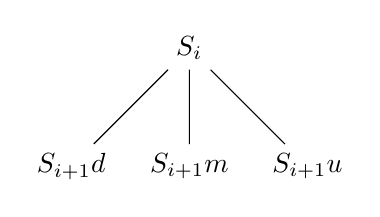
\begin{tikzpicture}[
  level 1/.style={},
  level 2/.style={},
  every node/.style={}
]
\node {\(S_i\)}
  child { node {\(S_{i+1}d\)}}
  child { node {\(S_{i+1}m\)}}
  child { node {\(S_{i+1}u\)}};
\end{tikzpicture}
\end{frame}

\begin{frame}{Matching Expectation and Variance of GBM}
Since
\[
\log (S_{t+\Delta t}) - \log(S_t) = 
\big(\mu -\frac{\sigma^2}{2}\big) \Delta t + \sigma W_{\Delta t},
\]
then $x_{i+1} - x_i$ satisfies
\[
\bE[ x_{i+1} - x_i] = \big(\mu -\frac{\sigma^2}{2}\big) \Delta t,  \quad \mathrm{Var}[x_{i+1} - x_i] = \sigma ^2 \Delta t.
\]
Matching conitnuous model and tree model gives
\[
\begin{cases}
p_u\Delta x_u + p_0 \cdot0 +p_d\Delta x_d&=\nu\Delta t,\\[4pt]
p_u\Delta x_u^2+ p_0 \cdot 0^2 + p_d\Delta x_d^2
&=\sigma^2\Delta t+\nu^2\Delta t^2,
\end{cases}
\]
where
\[
\nu=\mu-\frac12\sigma^2.
\]
\end{frame}

\begin{frame}{Q3: Derive trinomial probabilities}
By CRR model assumption,
\[
ud=1
\quad\Longrightarrow\quad
\Delta x_u=-\Delta x_d=:\Delta x.
\]
Solving the above linear system on $(p_u, p_d)$,
\[
\boxed{
p_u
=
\frac12\left(
\frac{\sigma^2\Delta t+\nu^2\Delta t^2}{\Delta x^2}
+
\frac{\nu\Delta t}{\Delta x}
\right)
}
\]
and
\[
\boxed{
p_d
=
\frac12\left(
\frac{\sigma^2\Delta t+\nu^2\Delta t^2}{\Delta x^2}
-
\frac{\nu\Delta t}{\Delta x}
\right).
}
\]
Finally, using
\(
p_u+p_0+p_d=1,
\)
we obtain
\[
\boxed{
p_0
=
1-
\frac{\sigma^2\Delta t+\nu^2\Delta t^2}{\Delta x^2}.
}
\]    
\end{frame}

\begin{frame}{Q6: Trinomial Tree Algorithm}

\begin{itemize}
\item Construct the terminal stock prices.
The log-price states at time \(t_n=T\) are
\[
x_{n,j}=\log S_0+j\Delta x,
\qquad
j=-n,-n+1,\ldots,n.
\]
\[
\boxed{
S_{n,j}
=
e^{x_{n,j}}
=
S_0e^{j\Delta x}.
}
\]
\item Apply the terminal payoff.
\[
\boxed{
V_{n,j}
=
(S_{n,j}-K)^+
=
\left(S_0e^{j\Delta x}-K\right)^+.
}
\]
\item Apply backward induction.
For
\[
i=n-1,n-2,\ldots,0,
\qquad
j=-i,-i+1,\ldots,i,
\]
\[
\boxed{
V_{i,j}
=
e^{-r\Delta t}
\left(
p_uV_{i+1,j+1}
+p_0V_{i+1,j}
+p_dV_{i+1,j-1}
\right).
}
\]
\end{itemize}
\end{frame}

\begin{frame}{Q6: Original Spacing Test}
\[
\Delta x=m\sqrt{2}\,\sigma\sqrt{\Delta t}.
\]

\begin{table}
\centering
\scriptsize
\setlength{\tabcolsep}{4.5pt}
\renewcommand{\arraystretch}{1.25}

\begin{tabular}{@{}lccccc@{}}
\toprule
\(m\backslash n\)
& \(20\) & \(60\) & \(100\) & \(140\) & \(180\)\\
\midrule

\(1/4\)
& \(-1.248\times10^{22}\)
& \(-4.548\times10^{68}\)
& \(-3.011\times10^{115}\)
& \(-2.376\times10^{162}\)
& \(-2.042\times10^{209}\)\\

\(1/2\)
& \(-2.344\times10^{8}\)
& \(-9.441\times10^{26}\)
& \(-6.879\times10^{45}\)
& \(-5.970\times10^{64}\)
& \(-5.644\times10^{83}\)\\

\(1\)
& \(8.5576172\)
& \(8.5802639\)
& \(8.5848161\)
& \(8.5867693\)
& \(8.5878551\)\\

\(2\)
& \(8.3279271\)
& \(8.5092001\)
& \(8.5426651\)
& \(8.5568032\)
& \(8.5646080\)\\

\(4\)
& \(7.2783882\)
& \(8.1778593\)
& \(8.3601143\)
& \(8.4306837\)
& \(8.4680670\)\\

\bottomrule
\end{tabular}
\end{table}

\begin{itemize}
    \item For \(m<1\), the coefficients are not valid probabilities,
    and the numerical solution becomes unstable.
    \item For \(m\geq1\), the prices converge towards the
    Black--Scholes value \(8.5916583\).
\end{itemize}
\end{frame}

\begin{frame}{Q6: Modified Spacing Test}
The spatial step is
\[
\Delta x=m\sigma\sqrt{3\Delta t}.
\]
\begin{table}
\centering
\scriptsize
\setlength{\tabcolsep}{4.5pt}
\renewcommand{\arraystretch}{1.25}
\begin{tabular}{@{}lccccc@{}}
\toprule
\(m\backslash n\)
& \(20\) & \(60\) & \(100\) & \(140\) & \(180\)\\
\midrule

\(1/4\)
& \(-2.293\times10^{18}\)
& \(-1.950\times10^{57}\)
& \(-3.008\times10^{96}\)
& \(-5.532\times10^{135}\)
& \(-1.108\times10^{175}\)\\

\(1/2\)
& \(-2.055\times10^{3}\)
& \(-5.132\times10^{11}\)
& \(-2.302\times10^{20}\)
& \(-1.230\times10^{29}\)
& \(-7.155\times10^{37}\)\\

\(1\)
& \(8.5220177\)
& \(8.5686318\)
& \(8.5778636\)
& \(8.5818113\)
& \(8.5840023\)\\

\(2\)
& \(8.1480384\)
& \(8.4598902\)
& \(8.5139432\)
& \(8.5365217\)
& \(8.5489299\)\\

\(4\)
& \(6.7937480\)
& \(7.9243246\)
& \(8.2207150\)
& \(8.3386664\)
& \(8.3995872\)\\

\bottomrule
\end{tabular}
\end{table}

\begin{itemize}
    \item For \(m=1/4\) and \(m=1/2\), the numerical values are
    negative and diverge as \(n\) increases.
    \item For \(m\geq1\), the method remains stable and converges
    towards the Black--Scholes value \(8.5916583\).
    \item A larger \(m\) gives a coarser spatial grid and slower convergence.
\end{itemize}
\end{frame}

\begin{frame}[fragile]{Q6: Python Code}
\begin{lstlisting}
def TOPM(n, dx):
    dt = T / n
    nu = r - 0.5 * sigma**2
    pu = 0.5 * ((sigma**2 * dt + nu**2 * dt**2) / dx**2 + nu * dt / dx)
    pd = 0.5 * ((sigma**2 * dt + nu**2 * dt**2) / dx**2 - nu * dt / dx)
    p0 = 1 - (sigma**2 * dt + nu**2 * dt**2) / dx**2
    values = np.array([max(S0 * exp(j * dx) - K, 0) for j in range(-n, n + 1)])
    for _ in range(n):
        values = exp(-r * dt) * (pd * values[:-2] + p0 * values[1:-1] + pu * values[2:])
    return values[0]
\end{lstlisting}
\end{frame}

\section[BS-Formula]{Black–Scholes Formula (Q4)}
\begin{frame}{Q4: call price}
Given
\[
S_0=K=100,\qquad r=0.05,\qquad \sigma=0.15,\qquad T=1,
\]
compute
\[
d_1=\frac{\log(S_0/K)+(r+\frac12\sigma^2)T}{\sigma\sqrt T}
=0.4083333333,
\]
\[
d_2=d_1-\sigma\sqrt T=0.2583333333.
\]
Then
\[
\boxed{
C_0=S_0\Phi(d_1)-Ke^{-rT}\Phi(d_2)\approx8.5916583121
=8.5917.
}
\]
\end{frame}

\begin{frame}{Q4: put-call parity}
For European options with the same $S_0,K,T$,
\[
C_0-P_0=S_0-Ke^{-rT}.
\]
Therefore
\begin{align*}
P_0
&=C_0-S_0+Ke^{-rT}\\
&=8.5916583121-100+100e^{-0.05}\\
&=\boxed{3.7146007622}.
\end{align*}
\end{frame}

\begin{frame}[fragile]{Q4: Python Code}
\begin{lstlisting}
def Black_Scholes_Model(S0=100,
                        K=100,
                        T=1,
                        r=0.05,
                        sigma=0.15):

    d1 = (log(S0 / K) + (r + 0.5 * sigma**2) * T) / (sigma * sqrt(T))
    d2 = d1 - sigma * sqrt(T)

    callPrice = S0 * normalcdf(d1) - K * exp(-r * T) * normalcdf(d2)
    putPrice = callPrice + K * exp(-r * T) - S0

    return d1, d2, callPrice, putPrice
\end{lstlisting}
\end{frame}

\section*{End}

\begin{frame}{}
\centering

\vfill

{\Huge\color{blue!70!black}\textbf{Thank You!}}

\vspace{1cm}

{\Large Questions?}

\vfill

\end{frame}

\end{document}